In this chapter we present the experimental setup which was 
used to test the transmition of encrypted data, as well as results 
related to the power efficiency of the sensors, the processing 
capabilities of the proposed solution and resilience towards 
flooding and DDoS attacks.

\subsection{Experimental setup}

The above mentioned tests were performed using a small network 
composed of 3 SparrowE wireless sensor nodes. In this setup, 
one of the SparrowE nodes was designated as the netowrk coordinator 
while the other two nodes were plain sensors, as it can be seen in 
the figure below:

\begin{figure}[ht] \centering
  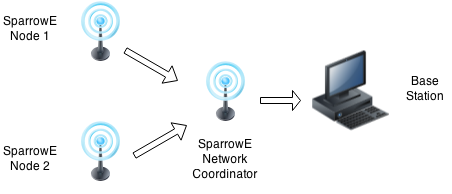
\includegraphics[width=0.5\textwidth]{img/experimental-setup.png}
  \caption{The SparrowE WSN experimental setup}
\end{figure}

The network coordinator is directly connected to the base station and 
its functions include analyzing incoming packets, decrypting the valid 
ones and passing the information on to the base station. The rest of the 
nodes are simply sensors which encapsulate and encrypt the data from their 
accelerometers and then broadcast it on the network.

\subsection{Software ECB and CBC efficiency}

The metric of interest is the number of encryption and decryption operations 
which can be performed in a unit of time by the software implementation of the 
ECB and CBC algorithms and if it scales linearly like the AES implementation does.

In order to gather the required data, both EBC and CBC have been performed on 
data from the node's sensors for periods of time lating 1, 2, 3, 4 and 5 seconds 
respectively. Then, the same was done using the AES implementations. The results 
can be observed in the tables shown below:

\\
\\

\captionof{table}{Number of operations performed by software/hardware ECB}
\begin{tabular}{ | l | p{1.5cm} | p{1.5cm} | p{1.5cm} | p{1.5cm} |}
    \hline
    Time & ECB Software Encryption & ECB Hardware Encryption & ECB Software Decryption & ECB Hardware Decryption \\ \hline
    1 & 901 & 3552 & 520 & 3550 \\ \hline
    2 & 1805 & 7105 & 1044 & 7101 \\ \hline
    3 & 2707 & 10661 & 1562 & 10653\\ \hline
    4 & 3604 & 14221 & 2084 & 14205\\ \hline
    5 & 4508 & 17761 & 2603 & 17752\\ \hline
\end{tabular}


\captionof{table}{Number of operations performed by software/hardware CBC}
\begin{tabular}{ | l | p{1.5cm} | p{1.5cm} | p{1.5cm} | p{1.5cm} |}
    \hline
    Time & CBC Software Encryption & CBC Hardware Encryption & CBC Software Decryption & CBC Hardware Decryption \\ \hline
    1 & 873 & 3550 & 509 & 3380 \\ \hline
    2 & 1747 & 7103 & 1023 & 6760 \\ \hline
    3 & 2623 & 10651 & 1530 & 10143 \\ \hline
    4 & 3495 & 14203 & 2038 & 13525 \\ \hline
    5 & 4367 & 17754 & 2546 & 16901\\ \hline
\end{tabular}

As it is seen in both tables, the results show that the software implementation, while 
slower than the hardware variant, scales linearly. The reduced number of operations which are 
performed in the software version does not represent a major drawback, as there is no immediate 
need to be able to process that amount of packets in one second. In fact, if a node were to send 
over 3000 packets in one second, the network would most likely be flooded.The main drawback of the 
software version is that the number of decryption operations performed is significantly lower than 
the number of encryption operations.

\subsection{Power consumption}

Under normal circumstances, the Atmega controller on the SparrowE nodes functions at a 
supply voltage of 3.6V and a frequency of 8MHz. If the nodes run the encryption by using 
only the software method, then the transceiver shall mostly be turned off while the sensor is 
running and its power consumption is negligible.

While performing encryption operations, it has been measured that the controller has a medium 
power consumption of 36mW, which can reach peaks of 50.4mW, meaning it normally uses a current 
of 10mA which spikes at 14mA. If the hardware approach is used and the tranceiver is turned on 
for large periods of time, it adds a power consumption of 1.63mW-3.48mW, meaning an average 
current of 490uA.

Because software encryption is performed slower than hardware encryption, the total consumption 
of both methods may be around the same average value. However, if performed at specific time 
intervals, software only operations can be more efficient from this point of view than the 
hardware equivalent.

\subsection{Flooding and DDoS protection}

Inside the wireless network running at 900MHz, the nodes communicate by broadcasting packets.
The network coordinator node shall receive and analyze any packet which arrives on this channel.
This opens up the risk of exposing the network to a DDoS attack. In order to determine how 
resilient the network is to such an attack and how much useful information the coordinator 
loses because it spends time analyzing and decrypting corrupt packets, such an attack has been 
simulated inside the experimental network.

The simulation is done by expanding the network to 5 nodes and having some of them transmit 
corrupt packets which are only meant to flood the network. The total size of these packets is 
112 bytes. The size must be a multiple of 16 in order to be processed by the block encryption 
algorithms. Then, these packets will be sent at time intervals starting at the network's default 
250ms and scaling down until the coordinator no longer receives any packets. The total number 
of packets sent during each iteration is 1500. The results can be seen in the figure below:

// ===================> plot cu packet loss

We can see that packet loss does not drastically increase in the interval of 250ms - 40ms. However, 
once we start sending packets once every 32ms or faster, the network becomes more and more flooded.
When the transmission interval reaches 20ms, the coordinator stops receiveing data. The overall packet
loss for the 5 sensor network transmitting at invervals of 250 milliseconds is 2 percent. 
